%preamble
\documentclass[letterpaper]{article}
\usepackage[utf8]{inputenc}
\usepackage[margin=1.25in]{geometry}

\usepackage{graphicx}
\graphicspath{{images/}}


\title{My Final Project}
\author{Deap Singh Bhandal}
\date{February 29 2020}

%the stuff for the document
\begin{document}
\maketitle
\section*{Abstract}
This project was inspired by the research from Cavender-Bares et al. and that team's reasearch on the live oak clade {\it Virentes}. I plan on expanding this section by introducing the results more. 

\newpage
\tableofcontents
\listoffigures
\newpage

\section{Introduction}
The study by Cavender-Bares et al. looked at several species of the American Live Oak clade which span North America and Mesoamerica. The researchers measured several variables from several oak trees in specific sites ranging from the genetic makeup of a specific tree to the climate the tree lives in\cite{cavender2004multiple}. While the researchers focused more on the genetic makeup differences between the tree species, I was more interested in the climate data. For one, there was an immense amount of data for each tree and I wanted to compare all the climate data variables to location, site, as well as characteristics of the tree such as foliar area. 
I was motivated to dig deeper into this since the researchers did not touch too much on the relationship between all the climate data and characteristics of the tree. I also recently took a class on plants and learned that depending on the climate, a tree’s leaf area index can range from under 1 to over 12\cite{jolly2005generalized}. The leaf area index is also known as foliar area which the researchers measured.

\section{Materials \& Methods}
I mainly used five functions in python to open, extract, manipulate, and close my data file. Each function is under it's own subsection. The outputs of the functions can be found in the Results section.
\subsection{Finding all the Locations}
\begin{verbatim}
# setting up a function that will print only the unique names from the Location list
def unique(file, num=1): 
    # opening data file
    data_file = open(file)
    # importing pandas
    import pandas as pd
    # assigning tmp_data variable to pandas file
    tmp_data = pd.read_csv(data_file)
    # assigning data variable to numpy file
    data = tmp_data.to_numpy()
    # Creating a list called cols that contains all the data from the col
    cols = (data[:, num]).tolist()
    # new empty list
    unique_list = [] 
    # for any city in col
    for ii in cols: 
        # it will be appended to list if it's not in unique list
        if ii not in unique_list: 
            unique_list.append(ii)
    # closing the file
    data_file.close()
    # returns the list
    return unique_list

print(unique('Dataset.csv', 1)) # seeing the unique locations
\end{verbatim}
\subsection{Counting all the Instances of a Location and Species Pair}
\begin{verbatim}
# setting a function that will count occurances of two values in two columns
def count_pair(file, numb1=1, numb2=2):
    # opening data file
    data_file = open(file)
    # importing pandas
    import pandas as pd
    # assigning tmp_data variable to pandas file
    tmp_data = pd.read_csv(data_file)
    # assigning data variable to numpy file
    data = tmp_data.to_numpy()
    # creating a new list of lists called bicols that has data from 2 cols
    bicols = (data[:, [numb1,numb2]]).tolist()
    # converting list of lists to list of tuples so it is easier for the program to count. 
    bicols = [tuple(i) for i in bicols]
    check = False
    # need new empty list
    new_list = []   
    ii = 0
    # closing the file
    data_file.close()
    # for loop checking if entry in new_list exists.
    for x in bicols: 
        if x in new_list:   
            check = True
            continue
        # if entry is not there it will append it, 
	# if there, it will not re-append it but will increase the count of ii
        else: 
            ii = 0
            #
            for y in bicols: 
                if y[0] == x[0] and y[1] == x[1]: 
                    ii = ii + 1
            # printing the number of occurences only for entries with multiple occurences        
            if(ii > 1):  
                print(x, "-", ii) 
            new_list.append(x)  
    if check == False: 
        # let's me know if an entry does not repeat
        print("No repeats")

# ran program successfully on Location_Species
count_pair('Dataset.csv',1,2)
\end{verbatim}
\subsection{Plotting Foliar Area Verses all Climate Data}
\begin{verbatim}
def mass_plotting(file, xdata=1, ystart=2, yend=3):
    # opening data file
    data_file = open(file)
    # importing pandas
    import pandas as pd
    # assigning tmp_data variable to pandas file
    tmp_data = pd.read_csv(data_file)
    # assigning data variable to numpy file
    data = tmp_data.to_numpy()
    # importing matplotlib.pyplot as plt since I need it later
    import matplotlib.pyplot as plt
    # closing the file
    data_file.close()   
    # creating a list of all the column names located in header
    header_list = list(tmp_data)
    # since there are several columns describing the climate an individual tree is in,
    # and I want to compare foliar area to all of them, I made a function to 
    # plot Foliar Area vs. all of the climate columns
    # for loop searches through columns 19-57 which are the climate ones
    for column in range(ystart, yend):
        column_list = (data[:, [xdata,column]]).tolist()
        # made a list of tuples in [(x,y)] format
        column_list = [tuple(i) for i in column_list]
        xval = [x[0] for x in column_list]
        yval = [y[1] for y in column_list]
        # plotted with appropriate x and y labels
        plt.scatter(xval,yval)
        plt.xlabel(header_list[xdata])
        plt.ylabel(header_list[column])
        plt.show()

mass_plotting('Dataset.csv', 9, 19, 57)
\end{verbatim}
\subsection{Counting the Occurances of all Climate Values}
\begin{verbatim}
# A lot of the climate data had the same values since many came from the same area
# I want to count all the occurances for a value for all the climate data columns
# This function counts the occurances for columns 9-56, 
# and pushes the counts to a dictionary for each column
def count_to_dict(file, ystart, yend):
    # opening data file
    data_file = open(file)
    # importing pandas
    import pandas as pd
    # assigning tmp_data variable to pandas file
    tmp_data = pd.read_csv(data_file)
    # assigning data variable to numpy file
    data = tmp_data.to_numpy()
    # importing matplotlib.pyplot as plt since I need it later
    for column in range(ystart,yend):
        header_list = list(tmp_data)
        # for loop searches through columns 19-57 which are the climate ones
        column_list = tmp_data["{}".format(header_list[column])].tolist() 
	# {}.format used since column names change
        count_dict = dict() # new dict
        # for loop finds all the occurances of an element and 
	# assigns the value as frequency of the element (key)
        for ii in column_list:
            count_dict[ii] = count_dict.get(ii, 0) + 1
        # closing the file
        data_file.close()
        print(count_dict) # printing dict for one column
        print("\n") # helps to space them out

count_to_dict('Dataset.csv', 19, 57)
\end{verbatim}
\subsection{Using Regex to Count all the Occurances of Individuals' Codes}
\begin{verbatim}
# setting up a function that will count all the cases of a regex search command in a column
def regex_count(file, num=1, col_regex=r'\b[\w]+\b'):
    # importing re module
    import re
    # opening data file
    data_file = open(file)
    # importing pandas
    import pandas as pd
    # assigning tmp_data variable to pandas file
    tmp_data = pd.read_csv(data_file)
    # assigning data variable to numpy file
    data = tmp_data.to_numpy()
    # Creating a list called cols that contains all the data from the col
    cols = (data[:, num]).tolist()
    # converting column list to string
    cols_string = ' '.join(cols)
    # extracting all cases of the regex search
    find_regex = re.findall(col_regex, cols_string)
    # new empty list
    regex_list = []
    # appending all finds to empty list
    for ii in find_regex:
        regex_list.append(ii)
    # new empty dictionary
    regex_counts = dict()
    # keys will be regex and values will be occurances
    for iii in regex_list:
        regex_counts[iii] = regex_counts.get(iii, 0) + 1
    # sorting dictionary by value (occurances)
    sorted_regex_count = {k: v for k, v in sorted(regex_counts.items(), key=lambda item: item[1])}
    print(sorted_regex_count)
    # closing the file
    data_file.close()

# counting cases of all words in 'individual' column
regex_count('Dataset.csv', 7)
\end{verbatim}
\section{Results}
\subsection{All Locations}
\begin{verbatim}
['Baja', 'Mexico', 'Texas', 'Florida', 'Costa Rica (Mothers)', 'Honduras',
 'Belize', nan, 'Cuba', 'South Carolina', 'Louisiana', 'North Carolina']
\end{verbatim}
\subsection{Location and Species Pairs}
\begin{verbatim}
('Baja', 'BR') - 350
('Mexico', 'FU') - 656
('Texas', 'FU') - 92
('Florida', 'GE') - 289
('Florida', 'MN') - 126
('Costa Rica (Mothers)', 'OL') - 1028
('Honduras', 'OL') - 916
('Belize', 'OL') - 84
('Mexico', 'OL') - 1241
('Cuba', 'SA') - 120
('Florida', 'VI') - 475
('Texas', 'VI') - 34
('South Carolina', 'VI') - 100
('Louisiana', 'VI') - 60
('Mexico', 'VI') - 20
('North Carolina', 'VI') - 60
('Texas', 'HY') - 46
\end{verbatim}
\subsection{Foliar Area vs.Climate Data}
Please see Figures \ref{fig:Foliar_Area_vs_19} (on page \pageref{fig:Foliar_Area_vs_19}) to \ref{fig:Foliar_Area_vs_56} (on page \pageref{fig:Foliar_Area_vs_56}).
\subsection{Mode of each Climate Data Column}
I plan to refine my code further to only find the mode of each climate data as that might be more useful than seeing dictionaries for each column
\subsection{Occurances of Individuals' Codes}
I plan to refine my code further to be a list of tuples so it is easier to see in the document. 
\section{Discussion}
I plan to expand on the usefulness of any extracted data and the functions that allowed me to acheive that. 

\newpage

\bibliography{references}
\bibliographystyle{plain}

\newpage

\section*{Figures}

\begin{figure}[h]
\caption{Foliar Area vs Climate Data 19\label{fig:Foliar_Area_vs_19}}
\centering
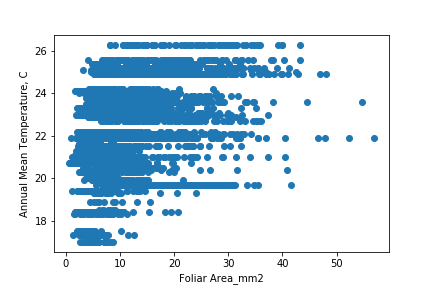
\includegraphics[width=0.7\paperwidth]{Foliar_Area_vs_19}
\end{figure}


\begin{figure}[h]
\caption{Foliar Area vs Climate Data 20\label{fig:Foliar_Area_vs_20}}
\centering
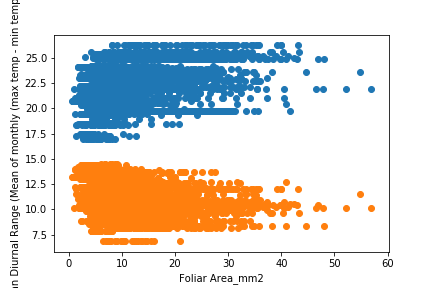
\includegraphics[width=0.7\paperwidth]{Foliar_Area_vs_20}
\end{figure}


\begin{figure}[h]
\caption{Foliar Area vs Climate Data 21\label{fig:Foliar_Area_vs_21}}
\centering
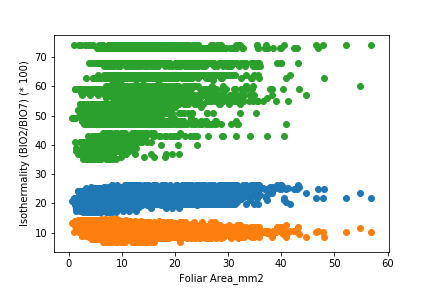
\includegraphics[width=0.7\paperwidth]{Foliar_Area_vs_21}
\end{figure}


\begin{figure}[h]
\caption{Foliar Area vs Climate Data 22\label{fig:Foliar_Area_vs_22}}
\centering
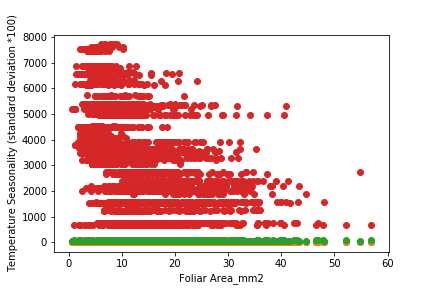
\includegraphics[width=0.7\paperwidth]{Foliar_Area_vs_22}
\end{figure}


\begin{figure}[h]
\caption{Foliar Area vs Climate Data 23\label{fig:Foliar_Area_vs_23}}
\centering
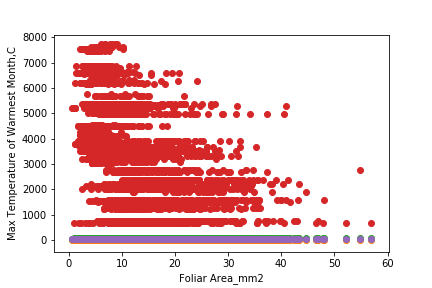
\includegraphics[width=0.7\paperwidth]{Foliar_Area_vs_23}
\end{figure}


\begin{figure}[h]
\caption{Foliar Area vs Climate Data 24\label{fig:Foliar_Area_vs_24}}
\centering
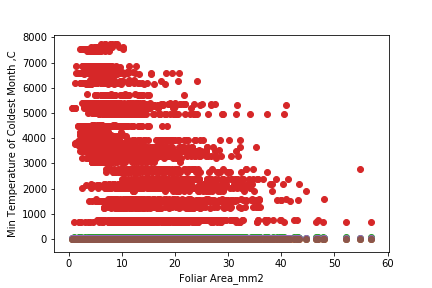
\includegraphics[width=0.7\paperwidth]{Foliar_Area_vs_24}
\end{figure}


\begin{figure}[h]
\caption{Foliar Area vs Climate Data 25\label{fig:Foliar_Area_vs_25}}
\centering
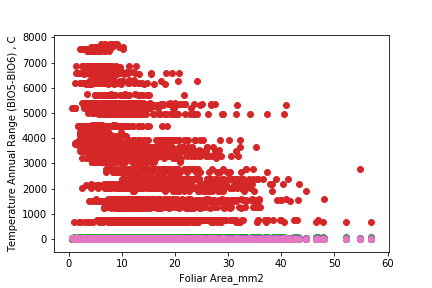
\includegraphics[width=0.7\paperwidth]{Foliar_Area_vs_25}
\end{figure}


\begin{figure}[h]
\caption{Foliar Area vs Climate Data 26\label{fig:Foliar_Area_vs_26}}
\centering
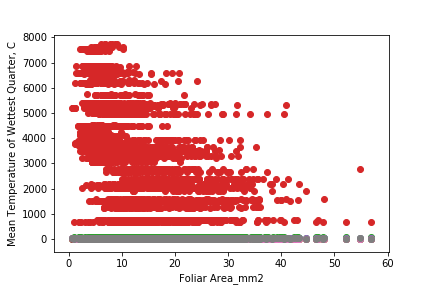
\includegraphics[width=0.7\paperwidth]{Foliar_Area_vs_26}
\end{figure}


\begin{figure}[h]
\caption{Foliar Area vs Climate Data 27\label{fig:Foliar_Area_vs_27}}
\centering
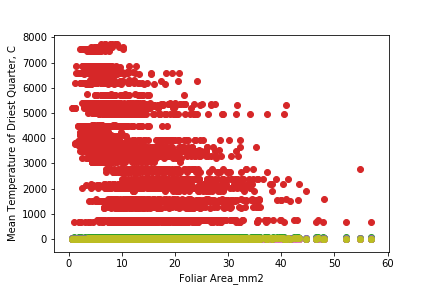
\includegraphics[width=0.7\paperwidth]{Foliar_Area_vs_27}
\end{figure}


\begin{figure}[h]
\caption{Foliar Area vs Climate Data 28\label{fig:Foliar_Area_vs_28}}
\centering
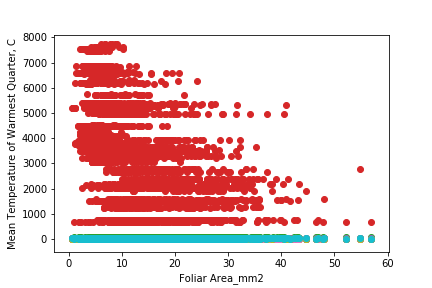
\includegraphics[width=0.7\paperwidth]{Foliar_Area_vs_28}
\end{figure}


\begin{figure}[h]
\caption{Foliar Area vs Climate Data 29\label{fig:Foliar_Area_vs_29}}
\centering
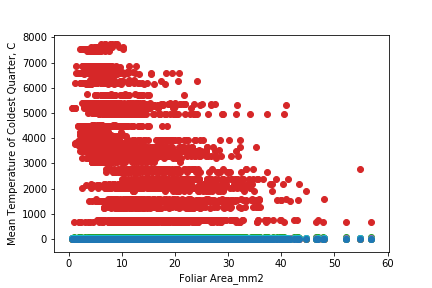
\includegraphics[width=0.7\paperwidth]{Foliar_Area_vs_29}
\end{figure}


\begin{figure}[h]
\caption{Foliar Area vs Climate Data 30\label{fig:Foliar_Area_vs_30}}
\centering
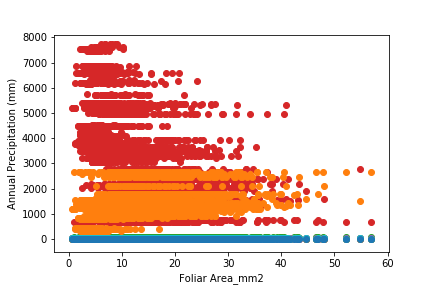
\includegraphics[width=0.7\paperwidth]{Foliar_Area_vs_30}
\end{figure}


\begin{figure}[h]
\caption{Foliar Area vs Climate Data 31\label{fig:Foliar_Area_vs_31}}
\centering
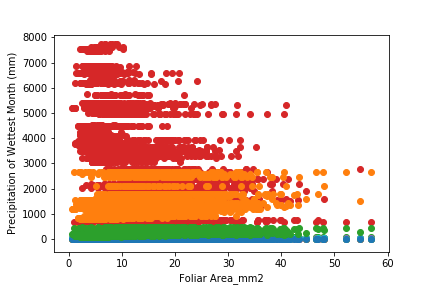
\includegraphics[width=0.7\paperwidth]{Foliar_Area_vs_31}
\end{figure}


\begin{figure}[h]
\caption{Foliar Area vs Climate Data 32\label{fig:Foliar_Area_vs_32}}
\centering
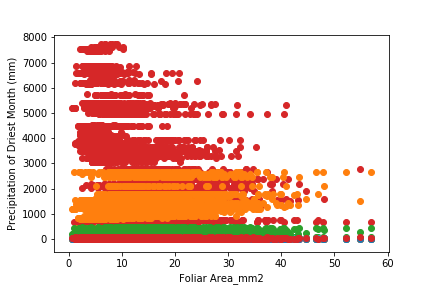
\includegraphics[width=0.7\paperwidth]{Foliar_Area_vs_32}
\end{figure}


\begin{figure}[h]
\caption{Foliar Area vs Climate Data 33\label{fig:Foliar_Area_vs_33}}
\centering
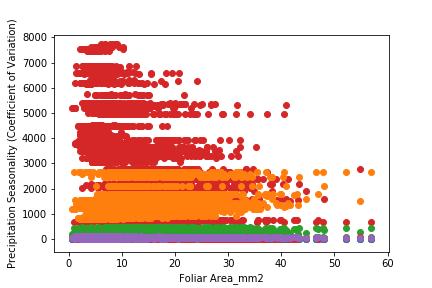
\includegraphics[width=0.7\paperwidth]{Foliar_Area_vs_33}
\end{figure}


\begin{figure}[h]
\caption{Foliar Area vs Climate Data 34\label{fig:Foliar_Area_vs_34}}
\centering
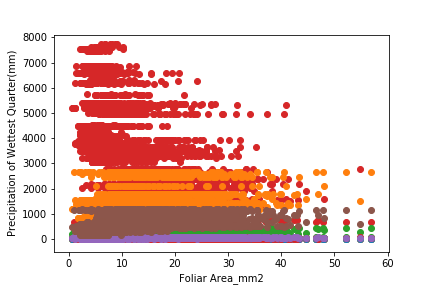
\includegraphics[width=0.7\paperwidth]{Foliar_Area_vs_34}
\end{figure}


\begin{figure}[h]
\caption{Foliar Area vs Climate Data 35\label{fig:Foliar_Area_vs_35}}
\centering
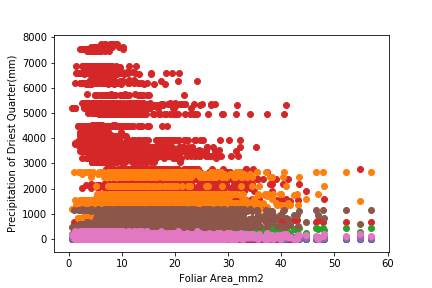
\includegraphics[width=0.7\paperwidth]{Foliar_Area_vs_35}
\end{figure}


\begin{figure}[h]
\caption{Foliar Area vs Climate Data 36\label{fig:Foliar_Area_vs_36}}
\centering
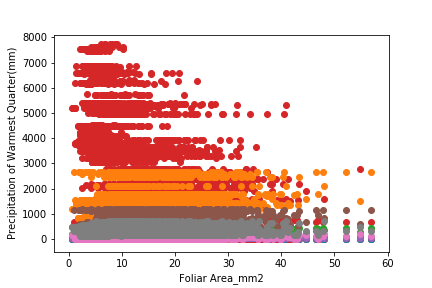
\includegraphics[width=0.7\paperwidth]{Foliar_Area_vs_36}
\end{figure}


\begin{figure}[h]
\caption{Foliar Area vs Climate Data 37\label{fig:Foliar_Area_vs_37}}
\centering
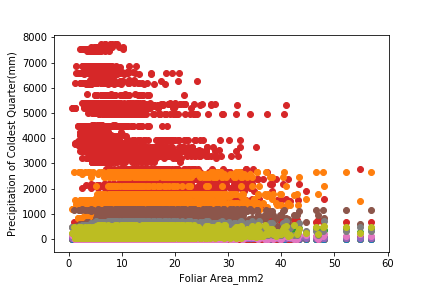
\includegraphics[width=0.7\paperwidth]{Foliar_Area_vs_37}
\end{figure}


\begin{figure}[h]
\caption{Foliar Area vs Climate Data 38\label{fig:Foliar_Area_vs_38}}
\centering
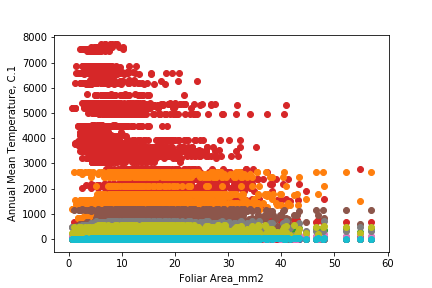
\includegraphics[width=0.7\paperwidth]{Foliar_Area_vs_38}
\end{figure}


\begin{figure}[h]
\caption{Foliar Area vs Climate Data 39\label{fig:Foliar_Area_vs_39}}
\centering
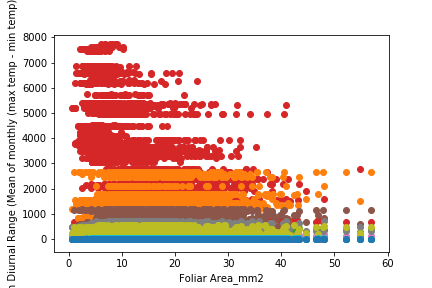
\includegraphics[width=0.7\paperwidth]{Foliar_Area_vs_39}
\end{figure}


\begin{figure}[h]
\caption{Foliar Area vs Climate Data 40\label{fig:Foliar_Area_vs_40}}
\centering
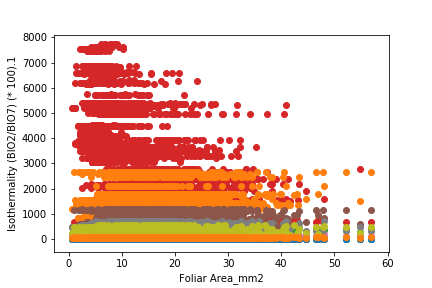
\includegraphics[width=0.7\paperwidth]{Foliar_Area_vs_40}
\end{figure}


\begin{figure}[h]
\caption{Foliar Area vs Climate Data 41\label{fig:Foliar_Area_vs_41}}
\centering
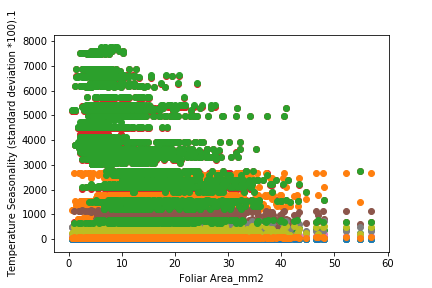
\includegraphics[width=0.7\paperwidth]{Foliar_Area_vs_41}
\end{figure}


\begin{figure}[h]
\caption{Foliar Area vs Climate Data 42\label{fig:Foliar_Area_vs_42}}
\centering
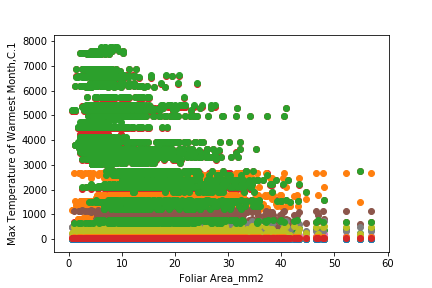
\includegraphics[width=0.7\paperwidth]{Foliar_Area_vs_42}
\end{figure}


\begin{figure}[h]
\caption{Foliar Area vs Climate Data 43\label{fig:Foliar_Area_vs_43}}
\centering
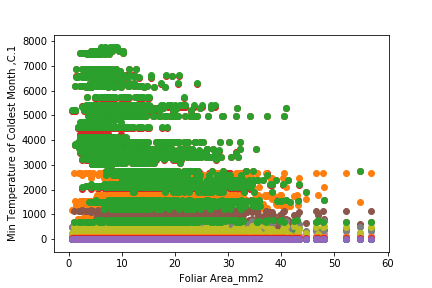
\includegraphics[width=0.7\paperwidth]{Foliar_Area_vs_43}
\end{figure}


\begin{figure}[h]
\caption{Foliar Area vs Climate Data 44\label{fig:Foliar_Area_vs_44}}
\centering
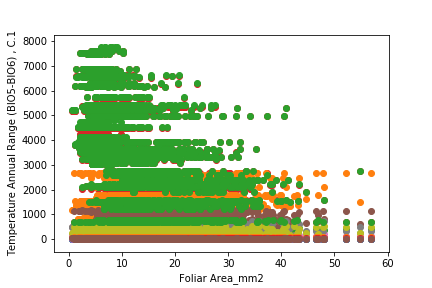
\includegraphics[width=0.7\paperwidth]{Foliar_Area_vs_44}
\end{figure}


\begin{figure}[h]
\caption{Foliar Area vs Climate Data 45\label{fig:Foliar_Area_vs_45}}
\centering
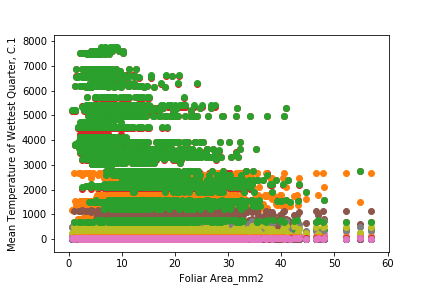
\includegraphics[width=0.7\paperwidth]{Foliar_Area_vs_45}
\end{figure}


\begin{figure}[h]
\caption{Foliar Area vs Climate Data 46\label{fig:Foliar_Area_vs_46}}
\centering
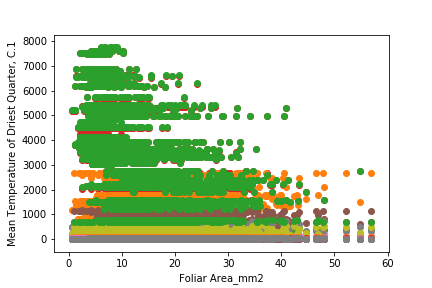
\includegraphics[width=0.7\paperwidth]{Foliar_Area_vs_46}
\end{figure}


\begin{figure}[h]
\caption{Foliar Area vs Climate Data 47\label{fig:Foliar_Area_vs_47}}
\centering
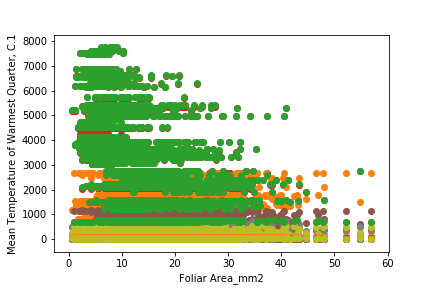
\includegraphics[width=0.7\paperwidth]{Foliar_Area_vs_47}
\end{figure}


\begin{figure}[h]
\caption{Foliar Area vs Climate Data 48\label{fig:Foliar_Area_vs_48}}
\centering
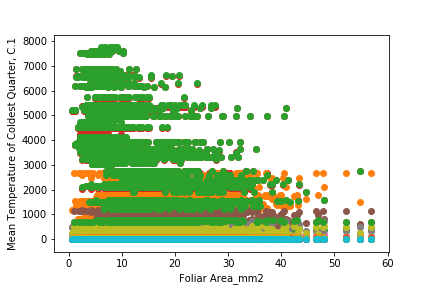
\includegraphics[width=0.7\paperwidth]{Foliar_Area_vs_48}
\end{figure}


\begin{figure}[h]
\caption{Foliar Area vs Climate Data 49\label{fig:Foliar_Area_vs_49}}
\centering
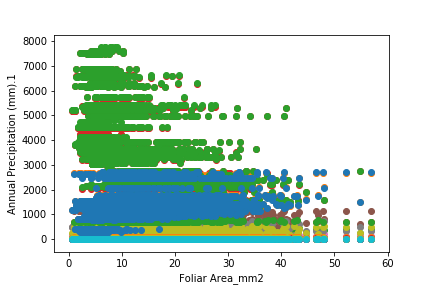
\includegraphics[width=0.7\paperwidth]{Foliar_Area_vs_49}
\end{figure}


\begin{figure}[h]
\caption{Foliar Area vs Climate Data 50\label{fig:Foliar_Area_vs_50}}
\centering
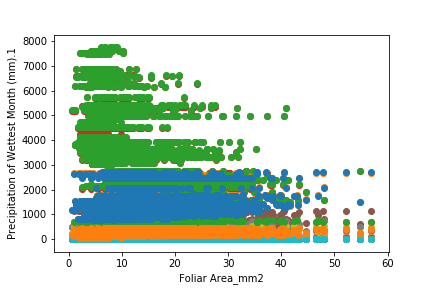
\includegraphics[width=0.7\paperwidth]{Foliar_Area_vs_50}
\end{figure}


\begin{figure}[h]
\caption{Foliar Area vs Climate Data 51\label{fig:Foliar_Area_vs_51}}
\centering
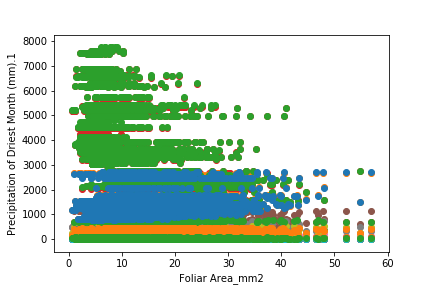
\includegraphics[width=0.7\paperwidth]{Foliar_Area_vs_51}
\end{figure}


\begin{figure}[h]
\caption{Foliar Area vs Climate Data 52\label{fig:Foliar_Area_vs_52}}
\centering
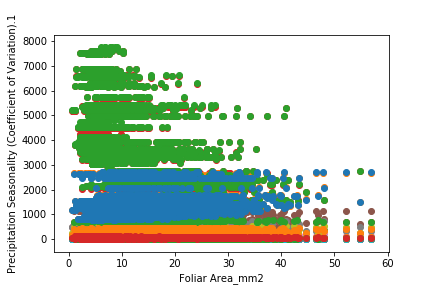
\includegraphics[width=0.7\paperwidth]{Foliar_Area_vs_52}
\end{figure}


\begin{figure}[h]
\caption{Foliar Area vs Climate Data 53\label{fig:Foliar_Area_vs_53}}
\centering
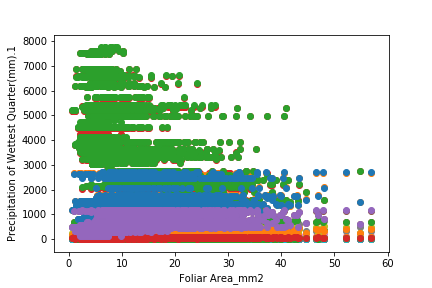
\includegraphics[width=0.7\paperwidth]{Foliar_Area_vs_53}
\end{figure}


\begin{figure}[h]
\caption{Foliar Area vs Climate Data 54\label{fig:Foliar_Area_vs_54}}
\centering
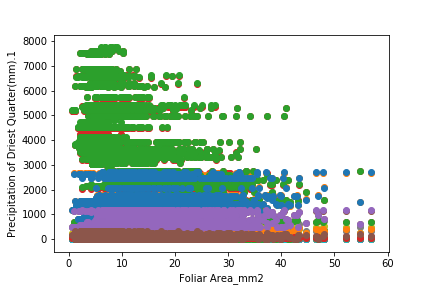
\includegraphics[width=0.7\paperwidth]{Foliar_Area_vs_54}
\end{figure}


\begin{figure}[h]
\caption{Foliar Area vs Climate Data 55\label{fig:Foliar_Area_vs_55}}
\centering
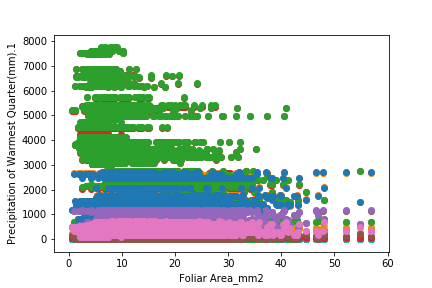
\includegraphics[width=0.7\paperwidth]{Foliar_Area_vs_55}
\end{figure}


\begin{figure}[h]
\caption{Foliar Area vs Climate Data 56\label{fig:Foliar_Area_vs_56}}
\centering
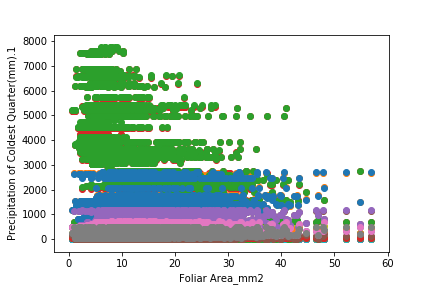
\includegraphics[width=0.7\paperwidth]{Foliar_Area_vs_56}
\end{figure}






\end{document}